\documentclass{article}
\usepackage{graphicx}
\graphicspath{ {figures/} }
\usepackage{enumitem}
\usepackage{hyperref}
\usepackage{comment}
\usepackage{xcolor}
\usepackage[utf8]{inputenc}
\usepackage[paper size={180mm, 240mm},left=25mm,right=25mm,top=35mm,bottom=25mm,nohea d]{geometry}
\usepackage{tabularx}
\usepackage{algpseudocode}
\usepackage{algorithm}
\usepackage{amsmath}
\usepackage{amssymb}


\usepackage{ltablex}

\usepackage{mdframed}
\usepackage{xcolor}
\surroundwithmdframed[
    hidealllines=true,
    backgroundcolor=black!20,
    skipbelow=\baselineskip,
    skipabove=\baselineskip
]{equation}

\usepackage{array}
\newcounter{rowcount}
\setcounter{rowcount}{0}
\newcommand\rownumber{\stepcounter{rowcount}\therowcount.}

%\renewcommand{\familydefault}{\sfdefault}%

\makeatletter
\def\namedlabel#1#2{\begingroup
    #2%
    \def\@currentlabel{#2}%
    \phantomsection\label{#1}\endgroup
}
\makeatother                                                               

\title{ Project Plan  
\\ ``MyTaxiService'' Application
\\ A.Y. 2015 - 2016 }

\author{Ennio Visconti (mat. 790382)
\\ Simone Zocchi (mat. 852910)
\\ Khanh Huy Paolo Tran (mat. 852496)}

\date{\today}
\makeatletter
\def\namedlabel#1#2{\begingroup
    #2%
    \def\@currentlabel{#2}%
    \phantomsection\label{#1}\endgroup
}
\makeatother

\bibliographystyle{plain}

\begin{document}
   
    \begin{titlepage}
        \maketitle 
        \vfill
        \centerline{
\includegraphics[scale=0.5]{LogoPolimi}}
        \vfill
        \vfill
    \end{titlepage}

        
    \tableofcontents

% --------------------------------------------------
% PLEASE REMEMBER TO UPDATE TIME SPENT IN time.tex
% --------------------------------------------------

\section{Introduction}

\subsection{Purpose}
This document has the \textbf{goal} of providing an overall and complete description of \textit{myTaxiService}'s software architectural design together with algorithms and UI.\\
The intended audience of this document are project managers and software developers.

\subsection{Scope}
\textit{myTaxiService} is an application born to support an existing taxi company, especially to simplify passengers' access to the service and guarantee a fair management of taxi queues. In fact it will be GPS-based and it will be able to assign a taxi to a certain call, based on the location of the taxi and of the requesting passenger, in order to minimize the waiting time.\\
It will also provide an option to reserve a taxi in advance and to share the ride with other passengers to save money. All these features will be available via a freely downloadable mobile application or a web application.\\
It will also provide an interface for the taxi drivers, in order to communicate with them more easily and to make them able to automatically share their location over time.

\subsection{Definitions, Acronyms, Abbreviations}

\subsubsection{Definitions}
\begin{itemize}
\item \textbf{Dynamic queue}: it is a list of taxis which is created whenever a request must be managed.
\item \textbf{Static queue}: it is a list of taxis which is associated to every zones. 
\end{itemize}

\subsubsection{Acronyms \& Abbreviations}
\begin{itemize}
\item \textbf{UML}: Unified Modeling Language
\item \textbf{API}: Application Programming Interface
\item \textbf{MVC}: Model - View - Controller
\item \textbf{DTO}: Data Transfer Object
\item \textbf{PSP}: Payment Service Provider
\end{itemize}


\subsection{Document Structure}
The document divides into 5 parts:
\begin{itemize}

\item Section 1: \textbf{Introduction}. It gives a description of the document underlining his goals and gives basic information about the application.

\item Section 2: \textbf{Architectural Design}. It gives the various architectural views of the application.

\item Section 3: \textbf{Algorithm Design}. It gives some algorithms' descriptions contained in the application.

\item Section 4: \textbf{User Interface Design}. It shows application's mockups.

\item Section 5: \textbf{Requirements Traceability}. It contains solutions to the RASD requirements.

\item Section 6: \textbf{References}. It contains all DD's references.

\end{itemize}



\section{Project size estimation - Function Points}
In this section the project size will be evaluated in terms of unadjusted function points. Given the following table summarizing the complexity weights of various function types, a detailed analysis will follow in the upcoming paragraphs.\\

\begin{figure}[h!]
        \centering
        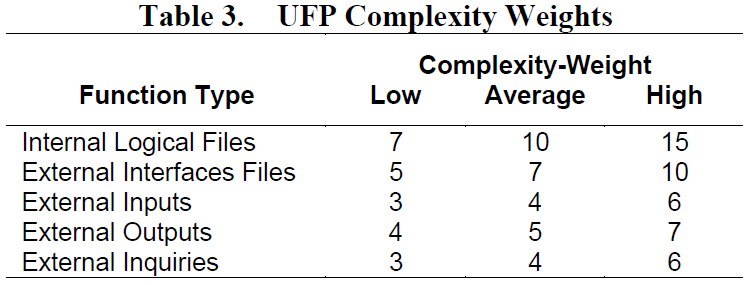
\includegraphics[width=0.7\columnwidth]{TabWeights2}
        \caption{Weights values}
        \label{fig:tw2}
\end{figure}

\subsection{INPUT}
    \paragraph {Passenger}
        \begin{itemize}
            \item \textbf{Login/Logout}: These operations con be considered with a \textit{Low} weight as they involve only one entity. 2 x 3 = \textbf{6 FPs}
            \item \textbf{Registration}: This operation involves a few more input data but still involves one entity, so it can be considered as \textit{Low} weight. 1 x 3 = \textbf{3 FPs}
            \item \textbf{Ride request / reservation}: These are quite complex, in fact they require some data from the user and the interaction with other entities. So consider these as \textit{High} weight. 2 x 6 = \textbf{12 FPs}
        \end{itemize}
    
    \paragraph{Taxi Driver}
        \begin{itemize}
            \item \textbf{Accept / Decline request}: This operation can be considered of \textit{Average} weight, as it requires only an interaction from the user, but in involves two other entities, request and passenger. 2 x 4 = \textbf{8 FPs}
            \item \textbf{Start / Stop ride}: Again this operation requires a single interaction from user, but involves other two entities, ride and Passenger. So we adopt an \textit{Average} weight. 2 x 4 = \textbf{8 FPs}
        \end{itemize}

\subsection{OUTPUT}
    \begin{itemize}
        \item \textbf{Total fare of a ride}: This operation requires information from three different entities, ride, driver and passenger, it can be considered of \textit{High} weight. 1 x 7 = \textbf{7 FPs}
        \item \textbf{Notification for accepted ride}: This operation requires information from two different entities, driver and passenger, it can be considered of \textit{Average} weight. 1 x 5 = \textbf{5 FPs}
        \item \textbf{Notification for ride request}: This operation requires information from three different entities, request, driver and passenger, it can be considered of \textit{High} weight. 1 x 7 = \textbf{7 FPs}
    \end{itemize}

\subsection{INQUIRY}
    \paragraph {Passenger}
        \begin{itemize}
            \item \textbf{Rides Log}: This operation requires data from Passenger and Rides. It is a quite easy operation so can be considered of \textit{Low} weight. 1 x 3 = \textbf{3 FPs}
        \end{itemize}
    
    \paragraph{Taxi Driver}
        \begin{itemize}
            \item \textbf{Notifications}: This operation requires data Requests and Driver entities but still remains an easy operation, so can be considered of \textit{Low} weight. 1 x 3 = \textbf{3 FPs}
            \item \textbf{Passengers on board}: This operation requires information Passengers, Rides and Driver entities so can be considered of \textit{High} weight. 1 x 6 = \textbf{6 FPs}
        \end{itemize}

\subsection{ILF}
The following entities will be used to store information needed for the application:
\textbf{Passengers}, \textbf{Taxis}, \textbf{Requests}, \textbf{Rides} and \textbf{Drivers}.
They all have a simple structure, except for the Request entity that is a little bit more complicated. So we assigned a \textit{Low} weight to all the entities, except for Request that has an \textit{Average} weight. 4 x 7 + 1 x 10 = \textbf{38 FPs}
\subsection{EIF}
    \begin{itemize}
        \item \textbf{GPS location}: This file contains the GPS coordinates of the vehicle. Can be considered with a simple structure so we assigned a \textit{Low} weight. 1 x 5 = \textbf{5 FPs}
        \item \textbf{Payment data}: This file contains data about the payment. It is quite simple so we assigned a \textit{Low} weight. 1 x 5 = \textbf{5 FPs}
        \item \textbf{Path data}: This is a complex structure acquired from the Google Maps API, we assigned an \textit{High} weight. 1 x 10 = \textbf{10 FPs}
    \end{itemize}

\subsection{Summary}
 {\renewcommand{\arraystretch}{1.5}

\begin{tabularx}{\textwidth}{X  r}
    \hline 
    \textbf{Function Type} & \textbf{Total FP}\\ 
    \hline 
    
    Input &  6 + 3 + 12 + 8 + 8 = 37 FPs\\
    \hline 
    Output & 7 + 5 + 7 = 19 FPs\\
    \hline
    Inquiry & 3 + 3 + 6 = 12 FPs\\
    \hline
    ILF & 38 FPs\\
    \hline
    EIF & 5 + 5 + 10 = 20 FPs\\
    \hline
    Total & 37 + 19 + 12 + 38 + 20 = \textbf{126 FPs}\\
    \hline
\end{tabularx}}

\section{Effort and Cost estimation - COCOMO}
In this section effort and costs of the project will be evaluated, in terms of month-person units. A detailed analysis of the scale and cost drivers will follow in the upcoming paragraphs, as defined in the COCOMO II estimation standard.\\

\subsection{Scale Drivers}
    \begin{itemize}
        \item \textbf{Precedentedness [PREC]}: This is the first Enterprise project developed by our team. However the team members are quite familiar with the Java language and basic language constructs and patterns. The level is therefore \textbf{low}.
        
        \item \textbf{Development Flexibility [FLEX]}: The customer only set general goals, without restricting the flow to specific processes. However, at an high level, the taxi reservation process is quite standardized, which therefore means the level is \textbf{high}.
        
        \item \textbf{Architecture/risk resolution [RESL]}: 
        The architecture/risk resolution requires a more in depth analysis of some specific points, in particular:
        \begin{itemize}
            \item The Risk Management Plan generally identifies critical risk items and establishes milestones for resolving them. Rating Level: Nominal.
            \item Schedule and budget have been set, but at some level of abstraction. Rating Level: Nominal.
            \item The percent of development schedule spent on the architecture is at a Nominal rating.
            \item Percent of required top software architects available: High.
            \item Tool support available to resolve risk items: Nominal.
            \item Level of uncertainty in key architecture drivers: High
            \item Number and criticality of risk items: 2-4 => Nominal.
            \\Overall rating: \textbf{High}
        \end{itemize}
        
        \item \textbf{Team cohesion [TEAM]}: The development team works really well and in harmony. Developers knew each other years before starting the project and there are practically no communication problems between them. So the level is \textbf{extra high}.
        
        \item \textbf{Process maturity [PMAT]}: Given the calculation KPAs, by doing an arithmetic approximation, the result of the EPML is 3: \textbf{High}.
        % KPA: 3 Always + 1 Frequently + 1 Half + 3 Rarely || + 5 Not Apply + 5 Don't Know
        % EPML: 5 x (3*100% + 1*75% + 1*50% + 3*1% ) / (100 * 8) = 2.675
        % PMAT Rating: 2: Nominal; 3: High
        
    \end{itemize}
    
\subsection{Cost Drivers}
    \begin{enumerate}
        \item \textbf{Required Software Reliability [RELY]}: Since the software simply replaces a manual procedure, no particular losses would be generated by a system failure. Rating Level: \textbf{Low}.
        
        \item \textbf{Data Base Size [DATA]}: Test data is considered to don't be particularly huge. Rating Level: \textbf{Nominal}.
        
        \item \textbf{Product Complexity [CPLX]}:
        The product complexity can be divided in some more specific topics. An overview of the specific ratings is presented below:
        \begin{itemize}
            \item Control Operations: High.
            \item Computational Operations: High.
            \item Device-dependent Operations: Nominal.
            \item Data Management Operations: High.
            \item User Interface Management Operations: Nominal.
        \end{itemize}
            
        So the average rating level is \textbf{High}.
        
        \item \textbf{Developed for Reusability [RUSE]}: The project development will be done with the idea of reusable components to the level of the project (there are no plans of other programs to develop which will interact with it). Rating level: \textbf{Nominal}.
        
        \item \textbf{Documentation Match to Life-Cycle Needs [DOCU]}: The most life-cycle needs are covered by previous documents. However some parts still need some more documentation. Rating Level: \textbf{Low}.
        
        \item \textbf{Execution Time Constraint [TIME]}: There are no particular constraints about the execution times, but still the application must respond quickly to user inputs. Rating Level: \textbf{High}.
        
        \item \textbf{Main Storage Constraint [STOR]}: Since only the database must be stored, a minimum part of the available storage will be used. Rating Level: \textbf{Nominal}.
        
        \item \textbf{Platform Volatility [PVOL]}: Most of the technologies are really stable and there is no perception of significant changes in less than one year. Rating Level: \textbf{Low}.
        
        \item \textbf{Analyst Capability [ACAP]}: The analysts are quite efficient in extracting the needed design and in cooperating to find the best architectural solutions. Rating Level: \textbf{High}.
        
        \item \textbf{Programmer Capability [PCAP]}: The programmers as a team ave a really effective communication and can cooperate really well. Rating Level: \textbf{Very High}.
        
        \item \textbf{Personnel Continuity [PCON]}: There are no information about the statistical personnel turnover. Rating Level: \textbf{Nominal}.
        
        \item \textbf{Application Experience [APEX]}: The team is composed by only beginners software engineers. Therefore there is practically no experience in the development of this kind of products at an enterprise level. Rating Level \textbf{Very Low}.
        
        \item \textbf{Platform Experience [PLEX]}: All team members have quite a basic comprehension and few experience of the chosen platform. Rating Level: \textbf{Low}.
        
        \item \textbf{Language and Tool Experience [LTEX]}: All team members are quite experienced with the Java language and the common tools usually used for developing programs in that context. Rating Level: \textbf{High}.
        
        \item \textbf{Use of Software Tools [TOOL]}: Given the semi-mature definition of the application life cycle, and the choice of a continuous integration tool, an effective tool set has been defined. Rating Level: \textbf{High}.
        
        \item \textbf{Multisite Development [SITE]}: The development is fully collocated. Rating Level: \textbf{Extra High}
        
        \item \textbf{Required Development Schedule [SCED]}: The development schedule is properly set without any particular stretch-outs or compressions. Rating Level: \textbf{Nominal}.
        
    \end{enumerate}
    
    \subsection{Summary}
    Given the effort ($\epsilon$) equation, which is:
    \begin{equation}
        \epsilon = A \times Size^E \times EAF
    \end{equation}
    
    Where:
    \begin{itemize}
        \item A = 2.94 as in COCOMO II.2000
        \item Size: actual size of the product to be developed in terms of KSLOC (thousands of Source Lines Of Code).
        \begin{equation}
            Size = \frac{UFP \times LF}{1000}
        \end{equation}
        Where LF = 46 SLOCs as for the avarage value of J2EE applications.
        
        \item E : Exponent derived from the five Scale Drivers, with
        \begin{equation}
            E = B + 0.01 \times \sum_{j=1}^5 SF_j
        \end{equation}
        With B = 0.91 as in COCOMO II.2000
        \item EAF : Effort Adjustment Factor derived from the Cost Drivers, with
        \begin{equation}
            EAF = \prod_{i=1}^N EM_i
        \end{equation}
    \end{itemize}
    
    
 {\renewcommand{\arraystretch}{1.5}

\begin{tabularx}{\textwidth}{X  X r}
    \hline 
    \textbf{Scale Factors} & \textbf{Rating Level} &\textbf{SF Value}\\ 
    \hline 
    PREC & Low & 4.96\\
    \hline 
    FLEX & High & 2.03\\
    \hline
    RESL & High & 2.83\\
    \hline
    TEAM & Extra High & 0.00\\
    \hline
    PMAT & Nominal & 4.68\\
    \hline
    \textbf{TOTAL (Sum)} &  & \textbf{14.5}\\
    \hline
    \caption{Scale Drivers Recap}\label{tab:sf-summary}\\
\end{tabularx}}


{\renewcommand{\arraystretch}{1.5}

\begin{tabularx}{\textwidth}{X  X r}
    \hline 
    \textbf{Cost Drivers} & \textbf{Rating Level} &\textbf{Effort Multiplier}\\ 
    \hline 
    RELY & Low & 0.92\\
    \hline 
    DATA & Nominal & 1.00\\
    \hline
    CPLX & High & 1.17\\
    \hline
    RUSE & Nominal & 1.00\\
    \hline
    DOCU & Low & 0.91\\
    \hline
    TIME & High & 1.11\\
    \hline
    STOR & Nominal & 1.00\\
    \hline
    PVOL & Low & 0.87\\
    \hline
    ACAP & High & 0.85\\
    \hline
    PCAP & Very High & 0.76\\
    \hline
    PCON & Nominal & 1.00\\
    \hline
    APEX & Very Low & 1.22\\
    \hline
    PLEX & Low & 1.09\\
    \hline
    LTEX & High & 0.91\\
    \hline
    TOOL & High & 0.90\\
    \hline
    SITE & Extra High & 0.80\\
    \hline
    SCED & Nominal & 1.00\\
    \hline
    \textbf{TOTAL (Product)} &  & \textbf{0.53}\\
    \hline
    \caption{Cost Drivers Recap}\label{tab:em-summary}\\
\end{tabularx}}

Therefore the estimated effort is:

\begin{equation}
        \epsilon = 2.94 \times (\frac{126\times 46}{1000})^{0.91+0.01\times 14.5} \times 0.53 = \textbf{9.95 person-month}
\end{equation}

with an estimated duration of:
\begin{equation}
        \delta = C \times \epsilon^{D+0.2\times(E-B)} = 
        3.67 \times 9.95^{0.28+0.2\times 0.01 \times 14.5} = 
        \textbf{7.5 months}
\end{equation}
\textit{Note: C = 3.67 and D = 0.28 as for COCOMO II.2000}\\\\
% C=3.67 | D = 0.28
And a (minimum) required number of people of:
\begin{equation}
        \pi = \lceil \epsilon / \delta \rceil = \textbf{2 persons}
\end{equation}

\section{Tasks identification}
In this section the main tasks of the project will be described with related duration and dependencies. Tasks are divided in terms of the activity (or super-task) they are related to and some milestones, described with deliveries versioning) are set.\\
\textit{Note: versions are also tracked as "releases" on the \href{https://github.com/zsimo93/myTaxyServiceTVZ}{GitHub repository}}. \\

\subsection{Requirement Analysis \& Specification}
{\renewcommand{\arraystretch}{1.2}

\begin{tabularx}{\textwidth}{|l X |l| l|}
    \hline 
    & \textbf{Task} & \textbf{Duration (days)}    & \textbf{Dependencies}     \\ 
    \hline 
    
    \rownumber & Scenarios identification            & 5  &     \\ \hline
    \rownumber & Goals collection                    & 10 & 1   \\ \hline
    \rownumber & Constraints analysis                & 10 & 1   \\ \hline 
    \rownumber & Interface requirements collection   & 7  & 2,3 \\ \hline 
    \rownumber & Functional requirements collection  & 7  & 2,3 \\ \hline 
    \rownumber & Use cases writing                   & 4  & 1   \\ \hline 
    \rownumber & Alloy verification                  & 4  & 5   \\ \hline
    
    % Milestone 1: RASD (v. 0.1)
    \textbf{v.0.1} & \textbf{Milestone: RASD}        &    &     \\ \hline
    
    \caption{Requirements Analysis \& Specification Tasks}\label{tab:rasd-tasks}\\    
\end{tabularx}


\subsection{Design \& Architecture Development}
{\renewcommand{\arraystretch}{1.2}
\begin{tabularx}{\textwidth}{|l X |l| l|}
    \hline 
    & \textbf{Task} & \textbf{Duration (days)}    & \textbf{Dependencies}      \\ 
    \hline 
    
    \rownumber & Main blocks design and definition                  & 2 &      \\ \hline 
    \rownumber & Front end components definition                    & 7 & 8    \\ \hline 
    \rownumber & Back end components definition                     & 7 & 8    \\ \hline 
    \rownumber & Architectural styles and design patterns selection & 5 & 9,10 \\ \hline
    \rownumber & Components interfaces and Public API design        & 7 & 10   \\ \hline 
    \rownumber & Requests handling analysis                         & 5 & 11   \\ \hline 
    \rownumber & Request arrival and ride notification analysis     & 5 & 11   \\ \hline 
    \rownumber & Fare algorithm design                              & 4 &      \\ \hline 
    \rownumber & Shared request algorithm design                    & 8 & 13   \\ \hline 
    
    % Milestone 2: DD (v. 0.2)
    \textbf{v.0.2} & \textbf{Milestone: DD}                         &   &      \\ \hline
    
    \caption{Design \& Architecture Development Tasks}\label{tab:dd-tasks}\\
\end{tabularx}}

\subsection{Implementation \& Testing}
{\renewcommand{\arraystretch}{1.2}
\begin{tabularx}{\textwidth}{|l X |l| l|}
    \hline 
    & \textbf{Task} & \textbf{Duration (days)}    & \textbf{Dependencies}     \\ 
    \hline 
    
    \rownumber & Personal tools and workspace setup           &  2  &       \\ \hline 
    \rownumber & Integration plan definition                  &  7  & 17    \\ \hline
    \rownumber & Team toolset initialization                  &  3  & 17,18 \\ \hline
    
    % Milestone 3: ITPD (v. 0.3)
    \textbf{v.0.3} & \textbf{Milestone: ITPD}                 &     &    \\ \hline
    
    \rownumber & Units development and testing                & 60  & 19 \\ \hline 
    \rownumber & Algorithms implementation                    & 15  & 19 \\ \hline
    \rownumber & Subsystem integration testing                & 20  & 20 \\ \hline
    \rownumber & System integration testing                   & 30  & 22 \\ \hline
    
    % Milestone 4: Implementation (v. 1.0)
    \textbf{v.1.0} & \textbf{Milestone: First Release}         &     &    \\ \hline
    
    \caption{Implementation \& Testing Tasks}\label{tab:itpd-tasks}\\
\end{tabularx}}

\subsection{Project Scheduling}
The Gantt chart with the scheduling of the project is available here:
\href{https://app.ganttpro.com/shared/token/c77f8506cec4fe6fe99a4299007540715c25ffefccfc4745993b29d11b9eb74e}{\textit{Gantt chart}}

\newpage
\textit{}

\section{Resource allocation}

In this section all the tasks are assigned to the members of the group. Assignments has been done taking into account both personal skills and time availability. Task identifiers are the ones defined in the previous section.  \\

{\renewcommand{\arraystretch}{1.5}
\begin{tabularx}{\textwidth}{|X | X|}
    \hline 
    \textbf{Group Member} & \textbf{Tasks assigned}\\ 
    \hline 
    
    Ennio Visconti              &  1, 3, 4, 8, 10, 12, 16, 17, 18, 19, 20, 21, 22, 23\\ \hline
    Simone Zocchi               &  1, 2, 5, 8, 10, 11, 14, 15, 17, 18, 19, 20, 22, 23\\ \hline
    Khanh Huy Paolo Tran        &  1, 6, 7, 8, 9, 11, 13, 15, 17, 18, 19, 20, 22, 23\\ \hline
    
    
    \caption{Task assignment }\label{tab:itpd-tasks}\\
\end{tabularx}}

\section{Risks identification}

{\renewcommand{\arraystretch}{1.5}

\begin{tabularx}{\textwidth}{| c  X | l | l|}
    \hline 
       & \textbf{Risk}                                                          & \textbf{Probability}  & \textbf{Effect}\\ 
    \hline 
    
    R1 & Member of the group are ill and this will cause a shift in the plan.   & Moderate       & Marginal\\
    \hline
    R2 & Change in requirements and design are proposed.                        & Moderate       & Critical\\
    \hline
    R3 & Architectural components cannot support the load of requests.          & Low            & Critical\\
    \hline
    R4 & Faults in external components used (i.e. Google Maps, PayPal)          & Low            & Catastrophic\\
    \hline
    R5 & Faults in architectural components                                     & Low            & Catastrophic\\
    \hline
    R6 & Underestimate development time                                         & Moderate       & Serious\\
    \hline
    
    
\end{tabularx}
\begin{tabularx}{\textwidth}{|c | X|}
    \hline 
    \textbf{Risk} & \textbf{Recovery Action}\\ 
    \hline 
    
    R1 & Organize tasks in resource allocation so that more overlapping are present. \\
    \hline
    R2 & Make a clear and traceable RASD and DD and project a flexible architecture, so that changing are less effective.\\
    \hline
    R3 & Project the physical architecture of the system so that it can be distributed and easily expandable. \\
    \hline
    R4 & Take into account different alternatives for external components and implement different interfaces for the different ones. It will be possible to change the components used easily.\\
    \hline
    R5 & Consider the possibility of redundancy of the most critical architectural components (for example Open Street Maps instead of Google Maps and Skrill instead of PayPal).\\
    \hline
    R6 & Investigate the possibility to buy already done component to be integrated in the application and not implemented from scratch.\\
    \hline
    
\end{tabularx}

}

\end{document}